\documentclass[border=12pt]{standalone}
\usepackage{tikz}
\usetikzlibrary{positioning, calc, arrows.meta, fit, backgrounds}

\definecolor{input}{HTML}{FCE0E1}
\definecolor{conv}{HTML}{BFE8C7}
\definecolor{flatten}{HTML}{F2F4C1}
\definecolor{merge}{HTML}{C7B8FF}
\definecolor{output}{HTML}{FFE2BB}

\begin{document}

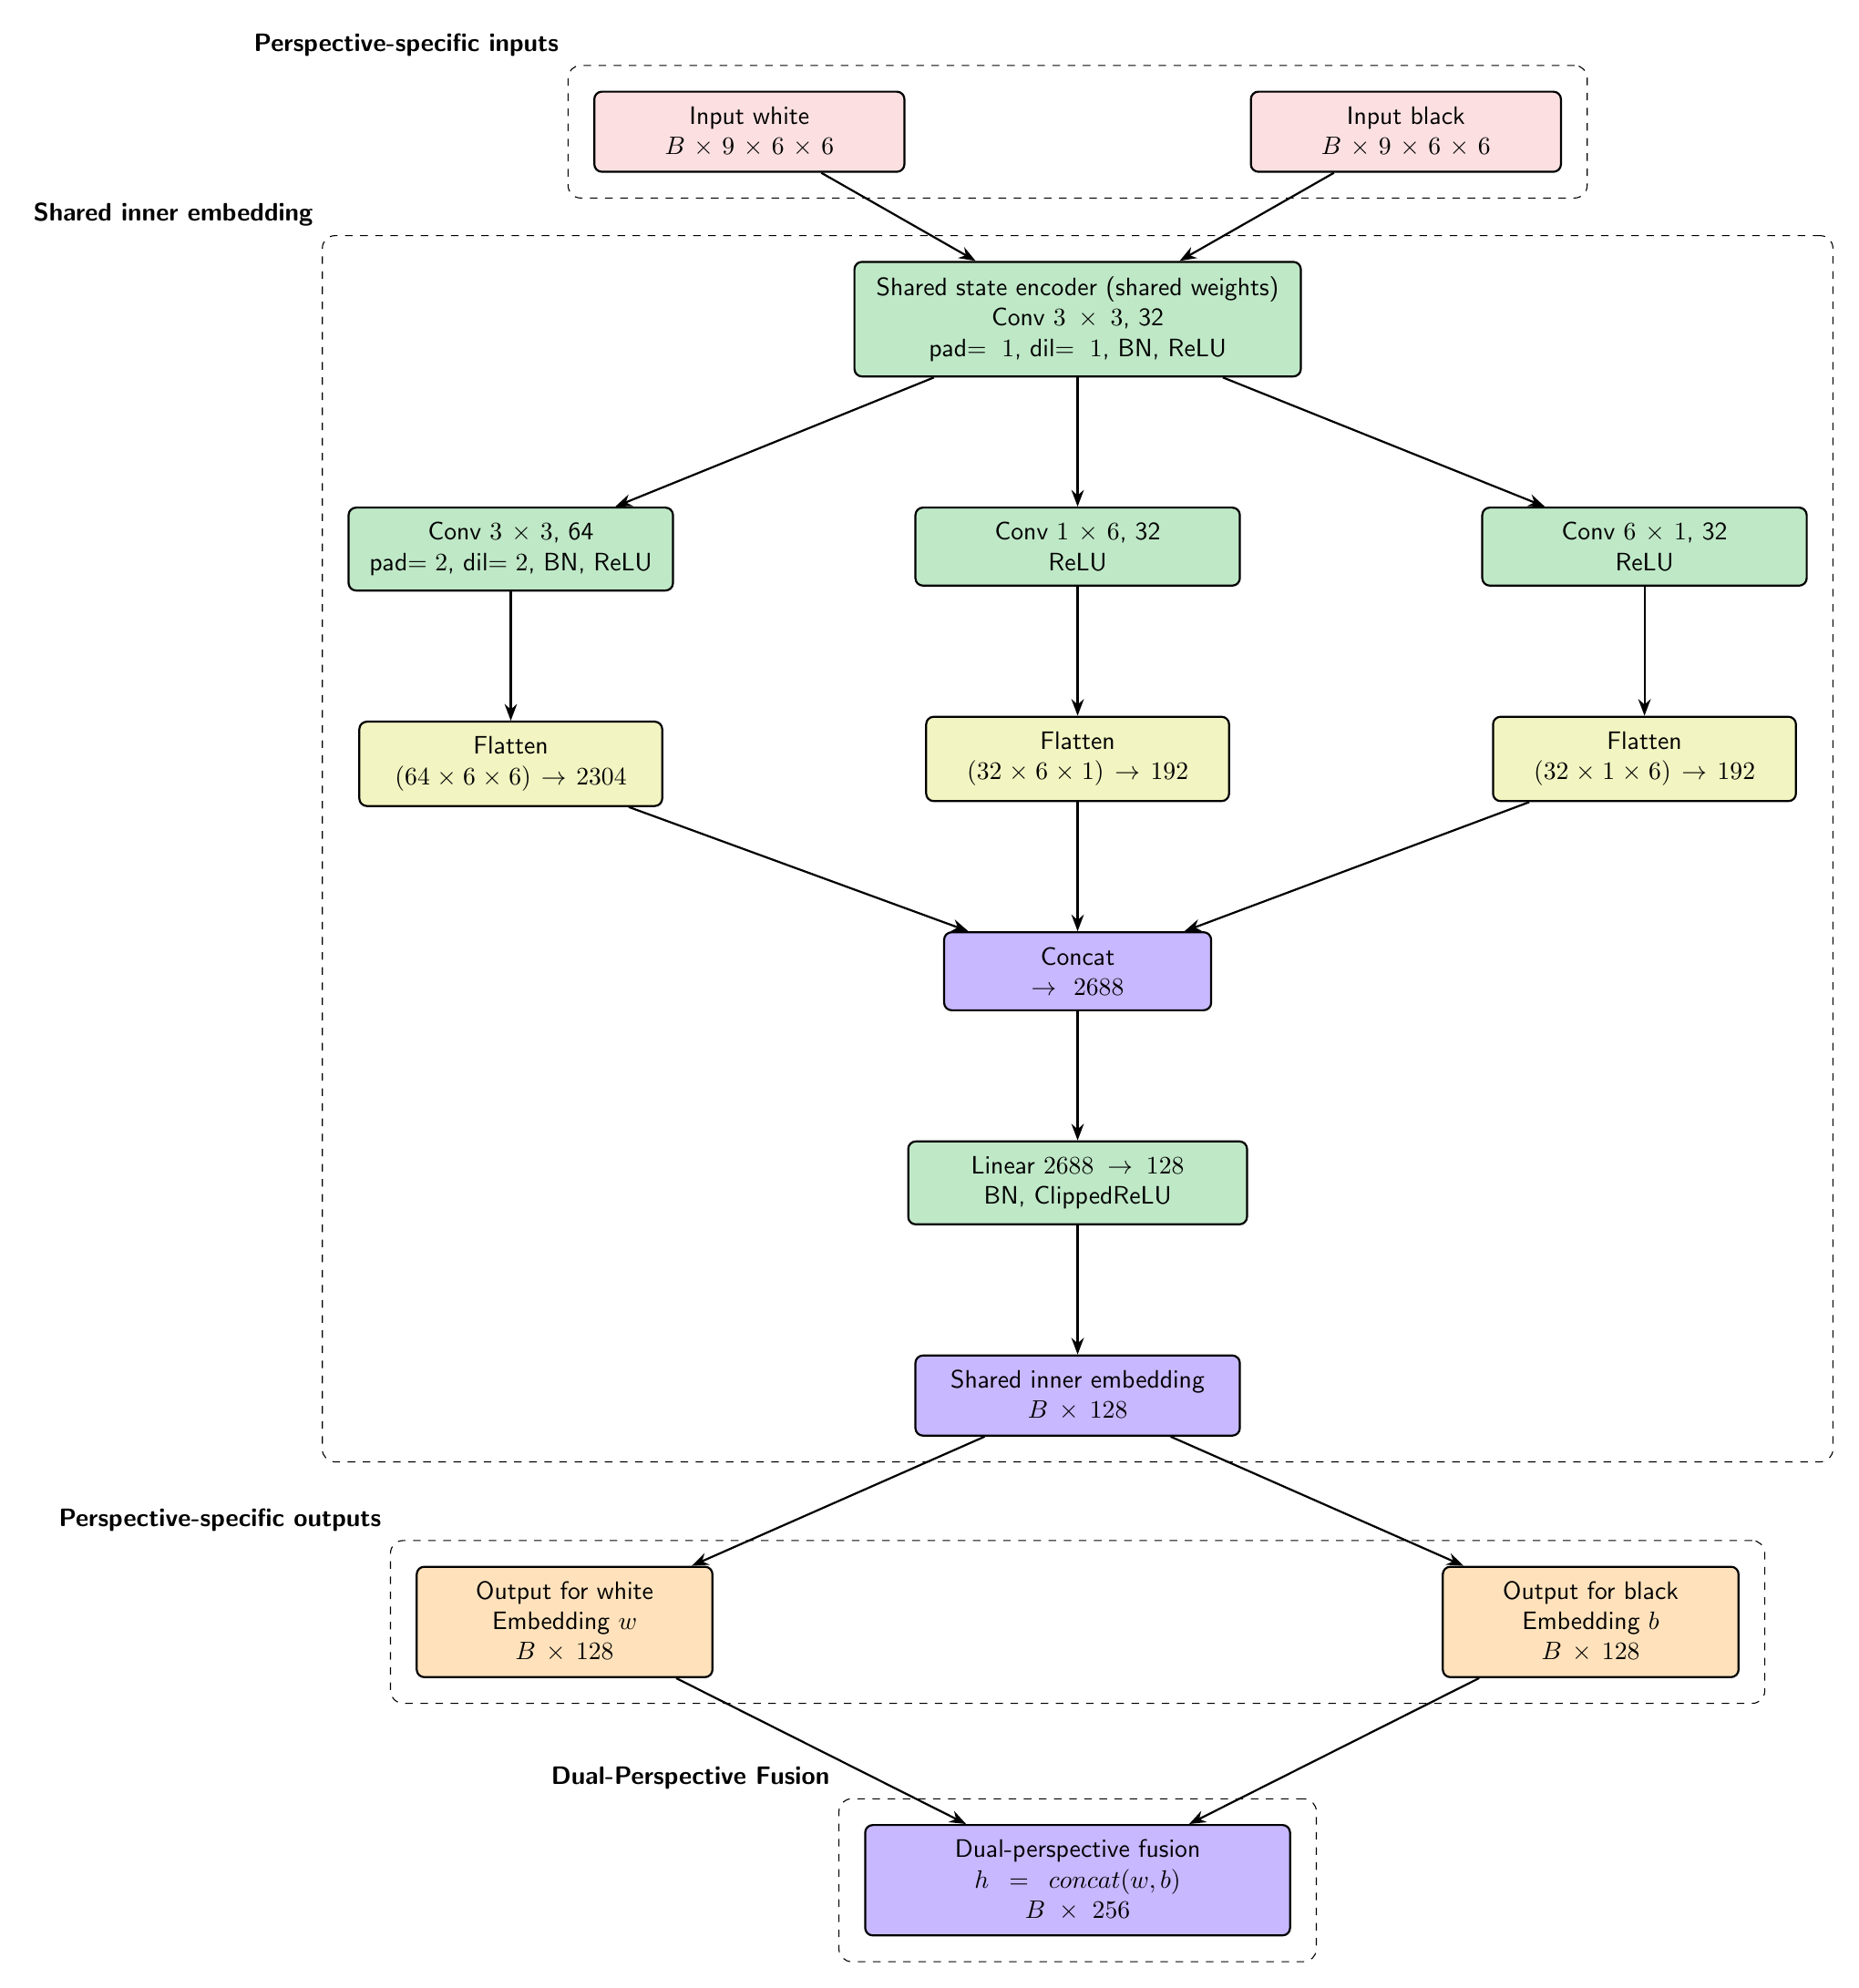
\begin{tikzpicture}[
    >=Stealth,
    thick,
    font=\sffamily,
    node distance=1.4cm and 1.6cm,
    block/.style={
        draw,
        rounded corners=3pt,
        align=center,
        minimum height=1.0cm,
        text width=4.5cm,
        inner sep=6pt
    },
    io/.style={block, fill=input},
    conv/.style={block, fill=conv},
    flat/.style={block, fill=flatten},
    merge/.style={block, fill=merge},
    output/.style={block, fill=output},
    groupbox/.style={
        draw,
        rounded corners=5pt,
        dashed,
        inner sep=10pt,
        label={[font=\bfseries\sffamily]north west:#1}
    }
]

\node[io, text width=3.9cm] (A1) {Input white\\$B \times 9 \times 6 \times 6$};
\node[io, right=4.8cm of A1, text width=3.9cm] (A2) {Input black\\$B \times 9 \times 6 \times 6$};

\node[conv, below=1.8cm of $(A1)!0.5!(A2)$, text width=5.8cm] (B) {Shared state encoder (shared weights)\\Conv $3\times 3$, 32\\pad$=1$, dil$=1$, BN, ReLU};

\node[conv, below left=1.8cm and 2.5cm of B, text width=4.1cm] (C) {Conv $3\times 3$, 64\\pad$=2$, dil$=2$, BN, ReLU};
\node[conv, below=1.8cm of B, text width=4.1cm] (D) {Conv $1\times 6$, 32\\ReLU};
\node[conv, below right=1.8cm and 2.5cm of B, text width=4.1cm] (E) {Conv $6\times 1$, 32\\ReLU};

\node[flat, below=1.8cm of C, text width=3.8cm] (F) {Flatten\\$(64 \times 6 \times 6) \rightarrow 2304$};
\node[flat, below=1.8cm of D, text width=3.8cm] (G) {Flatten\\$(32 \times 6 \times 1) \rightarrow 192$};
\node[flat, below=1.8cm of E, text width=3.8cm] (H) {Flatten\\$(32 \times 1 \times 6) \rightarrow 192$};

\node[merge, below=1.8cm of G, text width=3.3cm] (I) {Concat\\$\rightarrow 2688$};
\node[conv, below=1.8cm of I, text width=4.3cm] (J) {Linear $2688 \rightarrow 128$\\BN, ClippedReLU};
\node[merge, below=1.8cm of J, text width=4.1cm] (S) {Shared inner embedding\\$B \times 128$};

\node[output, below left=1.8cm and 2.8cm of S, text width=3.7cm] (K1) {Output for white\\Embedding $w$\\$B \times 128$};
\node[output, below right=1.8cm and 2.8cm of S, text width=3.7cm] (K2) {Output for black\\Embedding $b$\\$B \times 128$};

\node[merge, below=5.4cm of S, text width=5.5cm] (M) {Dual-perspective fusion\\$h=concat(w, b)$\\$B \times 256$};

\draw[->] (A1) -- (B);
\draw[->] (A2) -- (B);

\draw[->] (B) -- (C);
\draw[->] (B) -- (D);
\draw[->] (B) -- (E);

\draw[->] (C) -- (F);
\draw[->] (D) -- (G);
\draw[->] (E) -- (H);

\draw[->] (F) -- (I);
\draw[->] (G) -- (I);
\draw[->] (H) -- (I);

\draw[->] (I) -- (J);
\draw[->] (J) -- (S);
\draw[->] (S) -- (K1);
\draw[->] (S) -- (K2);
\draw[->] (K1) -- (M);
\draw[->] (K2) -- (M);

\begin{scope}[on background layer]
    \node[groupbox=Perspective-specific inputs, fit=(A1)(A2)] {};
    \node[groupbox=Shared inner embedding, fit=(B)(C)(D)(E)(F)(G)(H)(I)(J)(S)] {};
    \node[groupbox=Perspective-specific outputs, fit=(K1)(K2)] {};
    \node[groupbox=Dual-Perspective Fusion, fit=(M)] {};
\end{scope}

\end{tikzpicture}

\end{document}